% !TEX root = ../thesis.tex
In the HEFT, two diagrams will be necessary to match that in Fig. \ref{hbb2l}. The first one is shown in Fig. \ref{HEFTgloop} and is the contribution that intuitively comes to mind when one thinks of integrating out top quarks from the SM diagrams.
The addition of the diagram of Fig. \ref{HEFTbbtree} is a necessity: the one-loop diagram alone is UV divergent and requires a counter-term.
We will indeed see that the $H\bbbar$ coupling of the HEFT has a counter-term proportional to $C_{\text{ggH}}$.
Besides this divergent term, matching the expanded SM calculation to these two diagrams will also show that a finite term needs to be absorbed in the $H\bbbar$ coupling to reproduce the SM, which is the term we have set out to obtain.

\begin{figure}[!h]
  \centering
  \subfloat[]{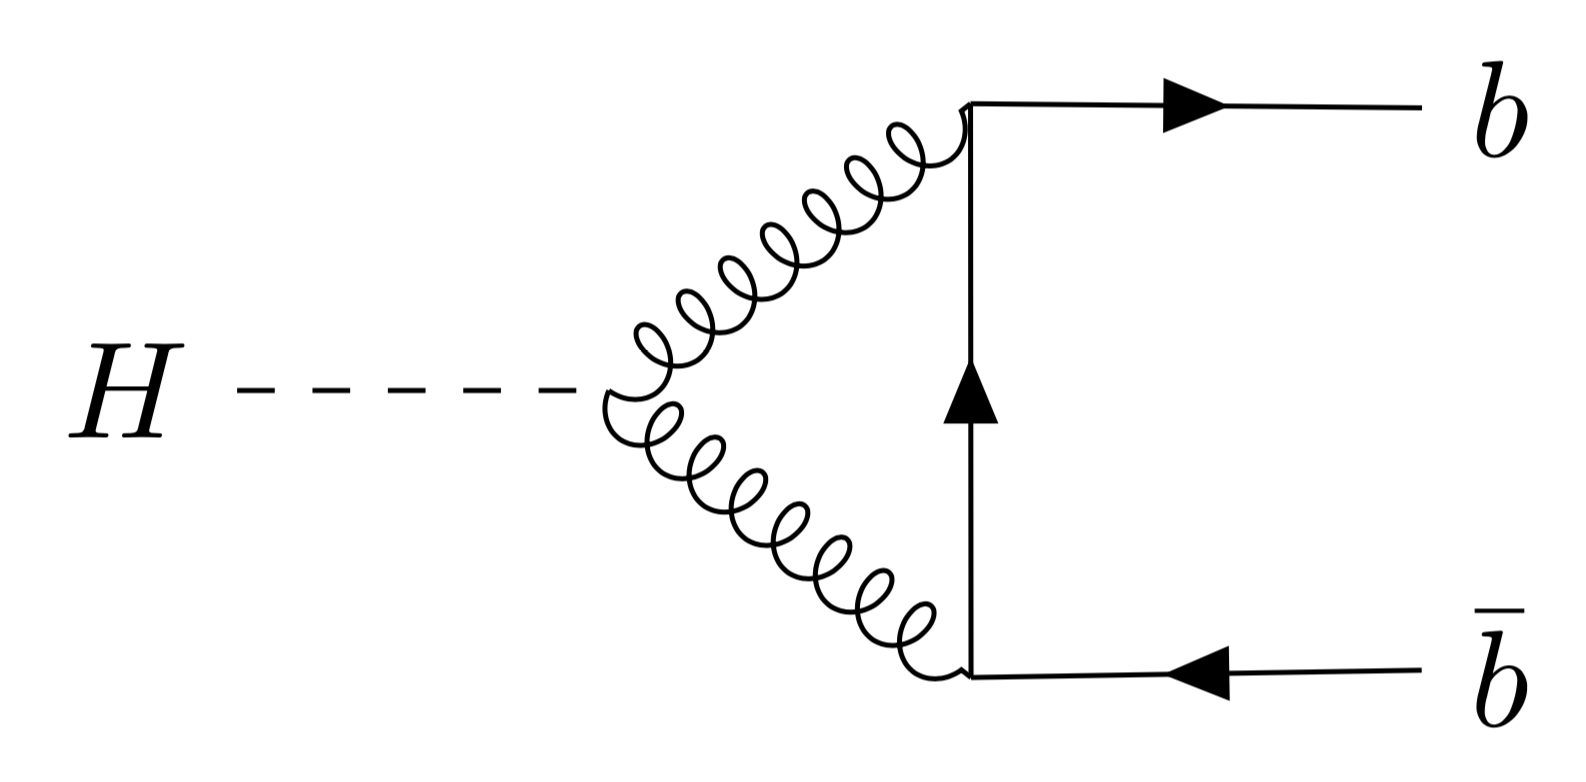
\includegraphics[height=7em]{Hbbgloop} \label{HEFTgloop}}\hspace{5em}
  \subfloat[]{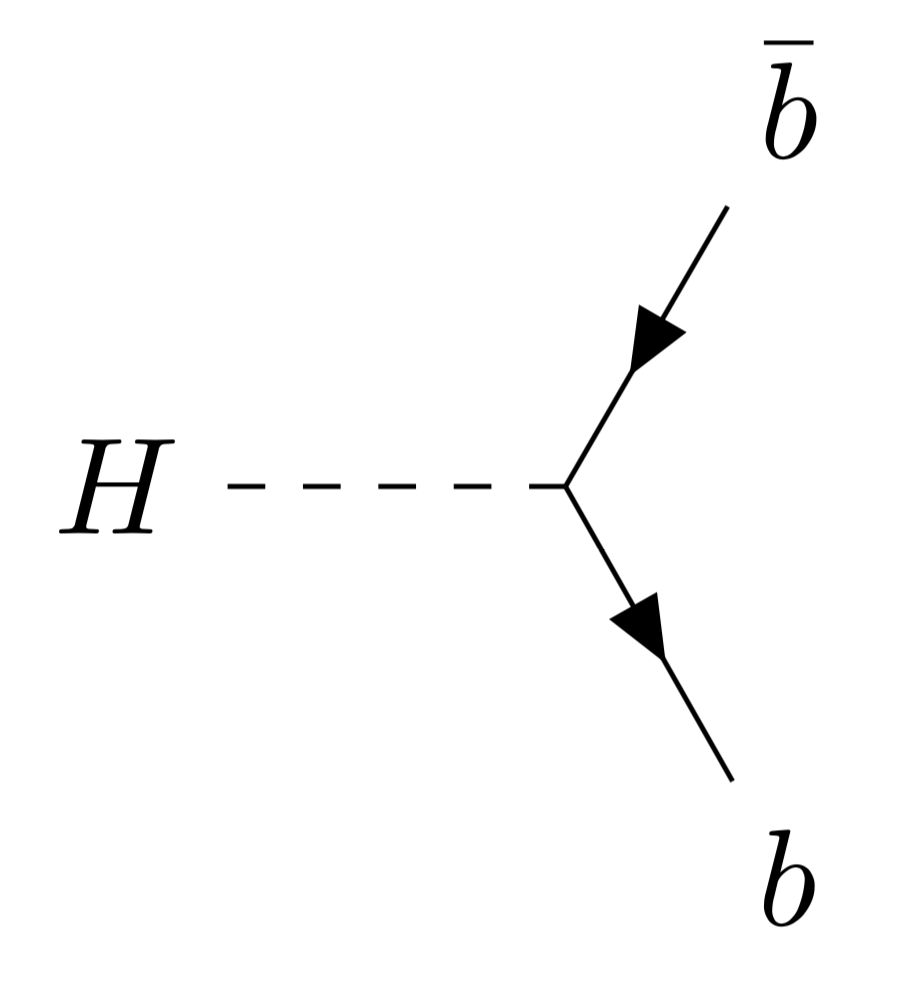
\includegraphics[height=8em]{Hbbtree}\label{HEFTbbtree}}\hspace{2em}
  \caption[$H\to\bbbar$ in the HEFT]{The two Feynman diagrams that contribute to $H\to \bbbar$ in the HEFT}
  \label{HEFThbbdiags}
\end{figure}

Another way to look at the presence of these two contributions will appear in the next section: the more complicated of the loop integrals that appear in the SM two-loop amplitude will have two regions in the $1/m_t$ expansion, which correspond to routing hard momenta through the top loop only or through the complete diagram.
These respectively have a diagramatical interpretation as shrinking the top loop in Fig. \ref{hbb2l} to obtain Fig. \ref{HEFTgloop} and shrinking the two loops to obtain Fig. \ref{HEFTbbtree}. This will be illustrated in the next section explicitly.

Since we wish to extract the power-suppressed corrections to a coupling that is present in the standard model, it is important that our notation makes a proper separation between the couplings in the SM and the HEFT to avoid confusion.
The interactions relevant for our calculation are the following:

\begin{table}[!h]
\begin{equation*}
{
  \renewcommand*{\arraystretch}{1.5}
  \begin{array}{ccc}
    \toprule
    \text{Coupling} & \text{Value} & \text{Feynman Rule}\\\midrule
     {\cal L}_{y_b} = - \frac{C_{y_b}}{\sqrt{2}}h\bar b b &C_{yb}=y_b+{\cal O}\left(\frac{1}{m_t}\right) & -i \frac{C_{y_b}}{\sqrt{2}}\\
     {\cal L}_{Hgg} = -\frac{1}{4}C_{Hgg} G_{\mu\nu}G^{\mu\nu}h & C_{Hgg}=\frac{\as}{3\pi v}& i C_{Hgg} \left( g^{\mu\nu} p_1\cdot p_2 - p_1^\nu p2^\mu \right)\footnote{Gluon 1: $(p_1,\mu)$, Gluon 2: $(p_2,\nu)$}  \\
     {\cal L}_{bG} = g_s G^\mu_a \bar b T^a\gamma_\mu b  & \text{Fixed by gauge invariance} & ig_s \gamma^\mu T^a \\
    \bottomrule
\end{array}}
\end{equation*}
  \caption[HEFT Lagragian and couplings]{HEFT interactions relevant for the calculation of the ${\cal O}(g_s^4 y_t)$ contribution to $H\to \bar b b$ and their leading-order values in the $1/m_t$ expansion.}
  \label{HEFTcoupligs}
\end{table}

Taken as it is, the amplitude $\cala_1$ associated with the diagrams in Fig. \ref{HEFThbbdiags} has external spinor wavefunctions and can be written as $\cala_1 = \bar u_b^\sigma(p_1) \cala_1^\text{amp} v_{\bar b}^{\sigma'}(p_2)$.

Since this calculation is a means to the end of extracting a Wilson coefficient, we don't need the full information and can project and spin average $\cala_1$ to get rid of the spinors. In practice, we will therefore work with

\begin{equation}
  \cala = \sum_{\sigma\sigma'} \bar v_{\bar b}^{\sigma'}(p_2) u_b^\sigma(p_1) \cala_1
  =\text{Tr}\left((\not p_1+m_b)\cala_1^\text{amp}(\not p_2-m_b)\right).
\end{equation}

The part of $\cala$ coming from Fig \ref{HEFTbbtree} is trivial to evaluate to find

\begin{equation}
  \cala_b = -i \frac{C_{y_b}}{\sqrt{2}}\left( s-4m_b^2 \right)
\end{equation}

We can now move on to the calculation of the one-loop diagram $\cala_\text{gf}$. Reading the Feynman rules, the expression is

\begin{equation}
  \cala_\text{gf} = i C_{Hgg} \left( i g_s  \right) \int \frac{d^dk}{(2\pi)^d} \frac{
  \text{Tr}\left((-i)(\not p_1+m_b) \gamma^\mu i(\not k +m_b)\gamma_\mu  (-i)(\not p_2-m_b)\right)
  }{\left( k+p_2 \right)^2 \left( k^2-m_b^2 \right) \left(k-p_1 \right)^2   }
\end{equation}

While this is a realtively simple amplitude, it is a good opportunity to illustrate the modern approach to loop calculations. Since there is only one diagram, choosing the topology is easy to define:

\begin{equation}
  \text{I}\left( n_1,n_2,n_3 \right) = \int\frac{d^dk}{(2\pi)^d} \frac{1}{D_1^{n_1}D_2^{n_2}D_3^{n_3}} =\int\frac{d^dk}{(2\pi)^d} \frac{1}{{  \left(\left(k-p_1 \right)^2\right)^{n_1}\left(\left( k+p_2 \right)^2\right)^{n_2}\left( k^2-m_b^2 \right)^{n_3}}}
\end{equation}

Whichs is summed up in Fig. \ref{hbbtopo}.

\begin{figure}[!h]
  \centering
  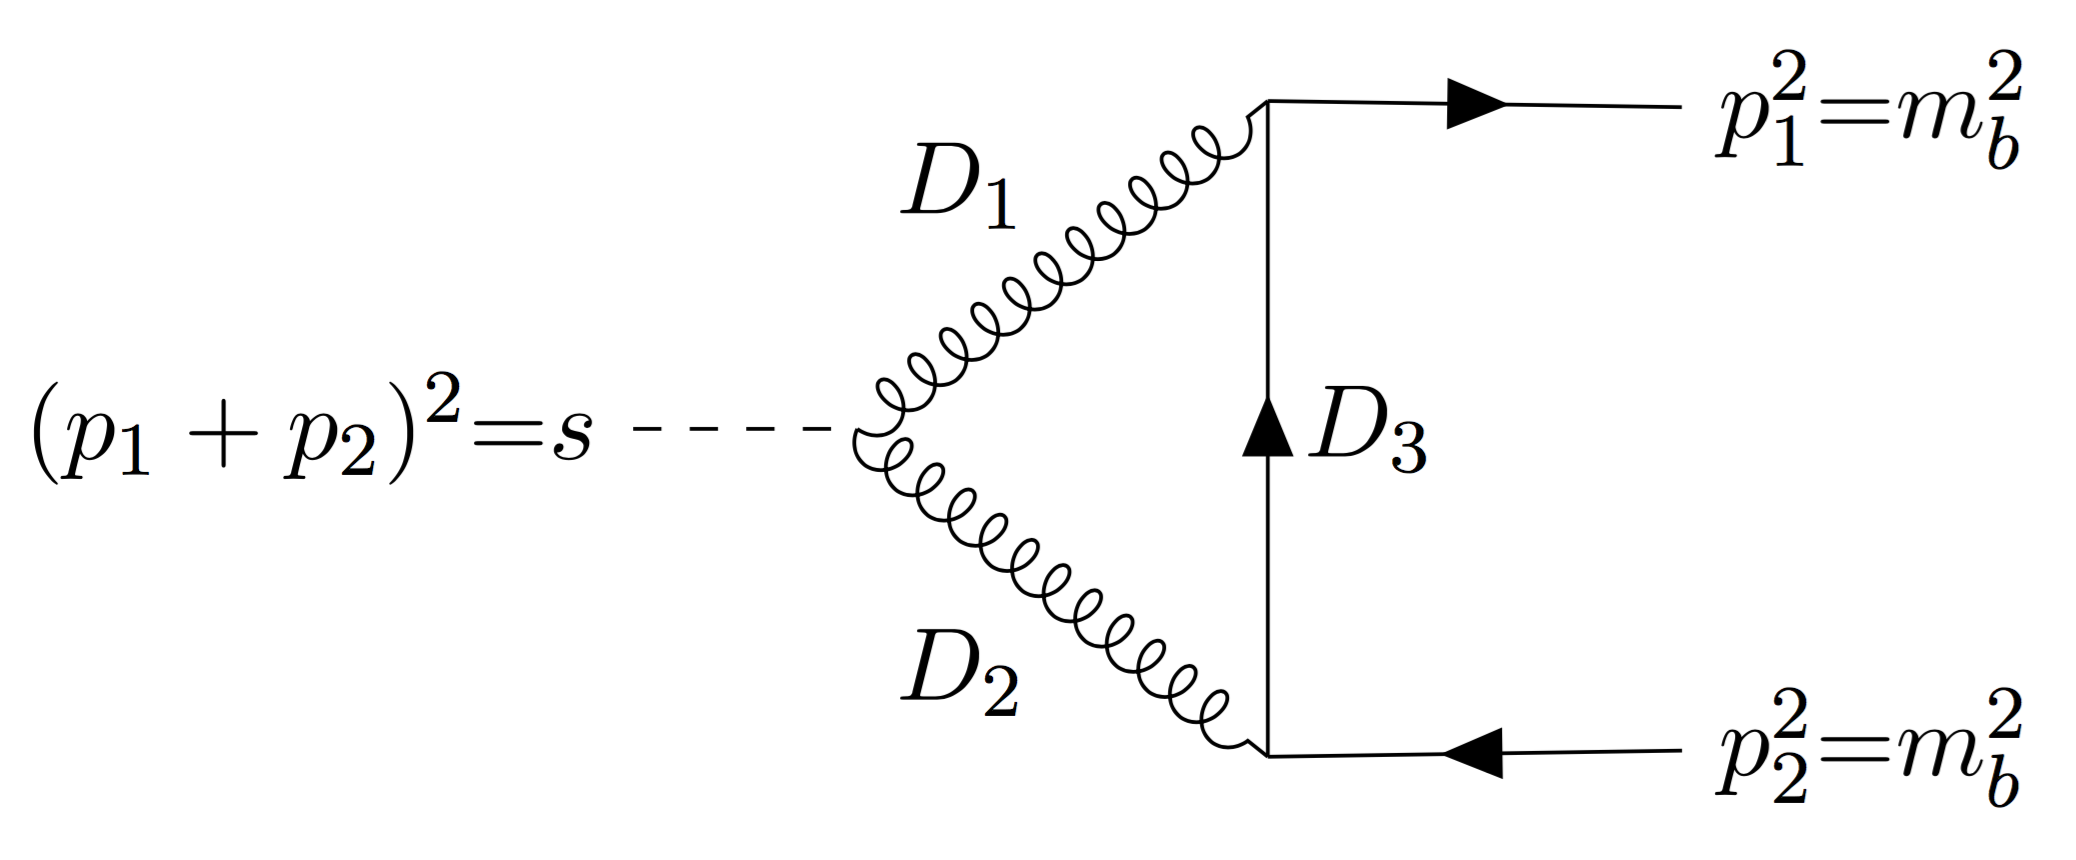
\includegraphics[width=0.6\textwidth]{hbbtopo}
  \caption{Graphical definition of the topology, defined as the set of denominators appearing in this diagram.}
  \label{hbbtopo}
\end{figure}

Reducing the integrals with numerators can be done using the following rules

\begin{equation}
k\cdot k = D_3^{-1}+m_b^2 ,\hspace{2em} k\cdot p_1 = \frac{D_3^{-1}-D_1^{-1}}{2}+m_b^2  ,\hspace{2em}  k\cdot p_2 = \frac{D_2^{-1}-D_3^{-1}}{2}-m_b^2.
\end{equation}

After calculating the trace and applying the rules, the diagram can be expressed as
\begin{equation}
\begin{split}
  \cala_{\text{gf}}=&
   -4 d s^2 \,\text{I}\left(1,1,1\right) m_b C_{Hgg}\, g_s^2
   -4 d \,\text{I}\left(-1,1,1\right) m_b C_{Hgg}\, g_s^2
   +8 d\,\text{I}\left(0,0,1\right) m_b C_{Hgg}\, g_s^2\\
&   -8 d \,\text{I}\left(0,1,0\right) m_b C_{Hgg}\, g_s^2
   +8 d s \,\text{I}\left(0,1,1\right)m_b C_{Hgg}\, g_s^2
   +8 d \,\text{I}\left(1,0,0\right) m_b C_{Hgg}\, g_s^2\\
&   -8 d s \,\text{I}\left(1,0,1\right) m_bC_{Hgg}\, g_s^2
   -4 d \,\text{I}\left(1,1,-1\right) m_b C_{Hgg}\, g_s^2
   +8 d s \,\text{I}\left(1,1,0\right) m_b C_{Hgg}\, g_s^2\\
&   +8 s^2 \,\text{I}\left(1,1,1\right) m_b C_{Hgg}\, g_s^2
   -32 \,\text{I}\left(0,1,1\right) m_b^3C_{Hgg}\, g_s^2
   -32 \,\text{I}\left(1,1,0\right) m_b^3 C_{Hgg}\, g_s^2\\
&   +32 s \,\text{I}\left(1,1,1\right) m_b^3 C_{Hgg}\, g_s^2
   +8 \,\text{I}\left(-1,1,1\right) m_b C_{Hgg}\, g_s^2
   -24 \,\text{I}\left(0,0,1\right) m_b C_{Hgg}\, g_s^2\\
&   +16 \,\text{I}\left(0,1,0\right) m_b C_{Hgg}\, g_s^2
   -16 s \,\text{I}\left(0,1,1\right) m_b C_{Hgg}\, g_s^2
   +16 \,\text{I}\left(1,-1,1\right) m_b C_{Hgg}\, g_s^2\\
&   -24 \,\text{I}\left(1,0,0\right) m_b C_{Hgg}\, g_s^2
   +40 s \,\text{I}\left(1,0,1\right) m_b C_{Hgg}\, g_s^2
   +8 \,\text{I}\left(1,1,-1\right) m_b C_{Hgg}\, g_s^2\\
&   -16 s \,\text{I}\left(1,1,0\right) m_b C_{Hgg}\, g_s^2
\end{split}
\end{equation}

This is a one-loop topology, so we know what the master integrals will look like: there can be triangle, bubble and tadpole integrals\footnote{Boxes are excluded because we only have three propagators}, and we will see this appear when reducing the family to a basis. For this topology, we used \code{FIRE5} to derive the IBP identities and reduce all the integrals in the amplitude to a set of three master integrals:

\begin{equation}
\setstretch{2.25}
{\renewcommand{\arraystretch}{2}
\begin{array}{rccrc}
\MI(1,1,1) & \raisebox{-2.5em}{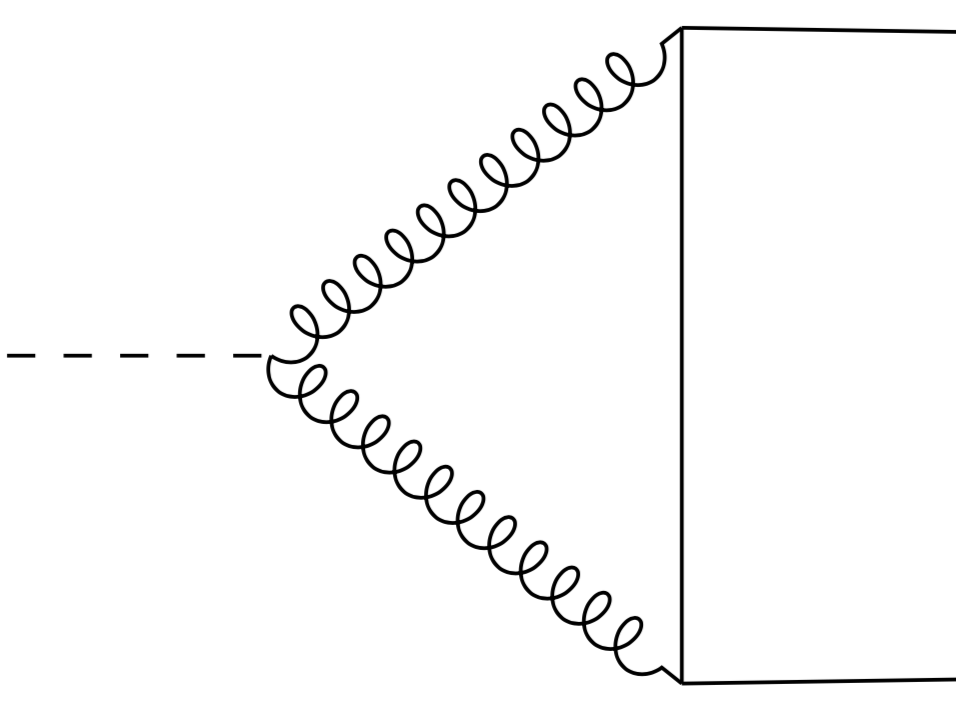
\includegraphics[height=5em]{hbb1ltriangle}} & \phantom{aaa}
\MI(1,1,0) & \raisebox{-2.5em}{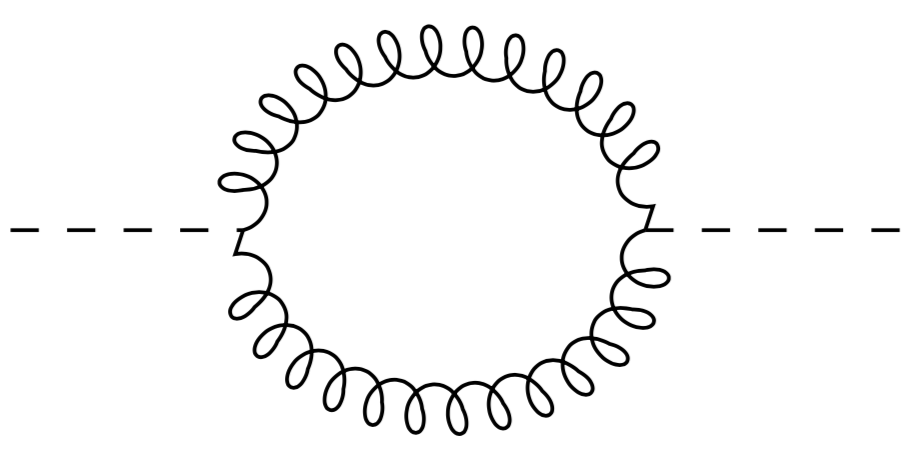
\includegraphics[height=5em]{hbb1lbubble}} \\
\MI(0,0,1) & \raisebox{-2.5em}{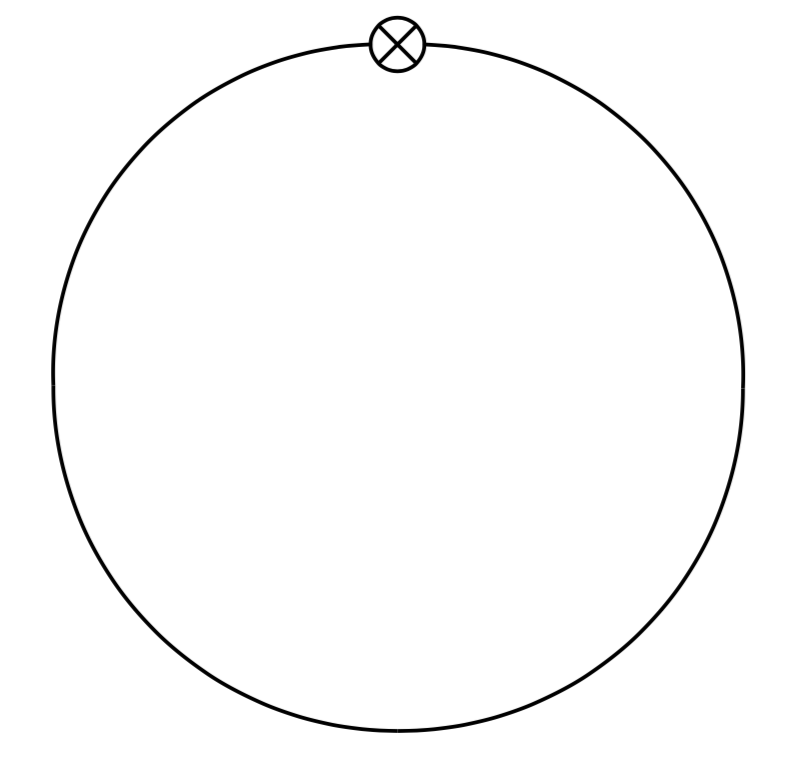
\includegraphics[height=5em]{hbb1ltadpole}}
\end{array}}
\end{equation}

These integrals can be directly evaluated by integrating their Feynman representations. They are of course well-known and can be found in a number of references (and textbooks for the tadpole and the bubble), but there is a pedagogic interest in illustrating how they can be evaluated.

\paragraph{Evaluation of the tadpole integral}

The easiest integral is the tadpole integral $\MI(0,0,1)$. We first need to evaluate its Feynman parametrization:

\begin{equation}
\MI(0,0,1)= \int\frac{d^dk}{(2\pi)^d} \frac{1}{k^2-m_b^2} = \int_0^1 dx \delta\left(1-x\right) i (4 \pi )^{-\frac{d}{2}} x^{1-d} \Gamma \left(1-\frac{d}{2}\right) \left(x^2 m_b^2\right){}^{\frac{d}{2}-1}
\end{equation}

No further work is required to find

\begin{equation}
  \MI(0,0,1)=i (4 \pi )^{-\frac{d}{2}} \Gamma \left(1-\frac{d}{2}\right) \left(m_b^2\right){}^{\frac{d}{2}-1}
\end{equation}

\paragraph{Evaluation of the bubble integral}

The bubble integral $\MI(1,1,0)$ requires slightly more work and in particular is a nice opportunity to showcase the role of the Cheng-Wu theorem in doing this kind of evaluation.

Let us first convert it to Feynman parametrization:

\begin{equation}
  \MI(1,1,0) = \int_0^\infty dx_1dx_2 \delta\left(1-x_1-x_2\right) i (4 \pi )^{-\frac{d}{2}} \left(x_1+x_2\right)^{2-d} \Gamma \left(2-\frac{d}{2}\right) \left(-s x_1 x_2\right){}^{\frac{d}{2}-2}
\end{equation}

This integrand is well-defined in the Euclidean region $s<0$. We will always perform integrations in this region and then analyticaly continuate to the region $s>0$ after integration. We can use the Cheng-Wu theorem to replace $\delta\left(1-x_1-x_2\right)$ by $\delta\left(1-x_2\right)$ and yield

\begin{equation}
\MI(1,1,0) = \int_0^\infty dx_1 i (4 \pi )^{-\frac{d}{2}} \left(1+x_1\right)^{2-d} \Gamma \left(2-\frac{d}{2}\right) \left(-s x_1\right){}^{\frac{d}{2}-2}.
\end{equation}

In which we can immediately identify an Euler beta function:
\begin{equation}
B(a,b)=\frac{\Gamma(a)\Gamma(b)}{ \Gamma(a+b) } = \int_0^\infty dz\, z^{a-1}(1+z)^{-a-b},
\end{equation}

and therefore

\begin{equation}
  \MI(1,1,0)=\frac{i (4 \pi )^{-\frac{d}{2}} (-s)^{\frac{d}{2}-2} \Gamma \left(2-\frac{d}{2}\right) \Gamma \left(\frac{d}{2}-1\right)^2}{\Gamma (d-2)}.
\end{equation}

\paragraph{Evaluation of the triangle integral}

The triangle integral $\MI(1,1,1)$ requires using more technology as it will involve multiple polylogarithms. It is important that we clearly identify this integral for the upcoming two-loop calculation we will perform in the Standard Model: we will see that in the $m_t\to\infty$ expansion, some two loop integrals appearing in the diagrams of Fig. \ref{hbb2l} will reduce to a form tadpole$\times$triangle. Identifying this is good for technical reasons as we can feed the result of this calculation into these integrals, but it also provides a very clear illustration of the how the matching between the two theories will work out.

The Feynman parametrization of this integral is

\begin{equation}
\MI(1,1,1)=\int dx_1dx_2dx_3 \delta \left( 1-x_1-x_2-x_3 \right) i (4 \pi )^{-\frac{d}{2}} \Gamma \left(3-\frac{d}{2}\right) \left(x_1+x_2+x_3\right){}^{3-d} \left(x_2^2 m_b^2-s x_1 x_3\right){}^{\frac{d}{2}-3}
\end{equation}

We can apply the Cheng-Wu theorem to eliminate $x_3$ and define the form of the triangle integral that we will match in further calculations

\begin{equation}
\begin{split}
\MI(1,1,1)=&\int_0^\infty dx_1dx_2 i (4 \pi )^{-\frac{d}{2}} \Gamma \left(3-\frac{d}{2}\right) \left(1+x_1+x_2\right){}^{3-d}  \left(m_b^2-s x_1 x_2\right){}^{\frac{d}{2}-3}\\
=& \int_0^\infty dx_1dx_2 i (4 \pi )^{-\frac{d}{2}}  \Gamma \left(3-\frac{d}{2}\right) m_b^{d-6} \left(1+x_1+x_2\right){}^{3-d} \left(1+r x_1 x_2\right){}^{\frac{d}{2}-3}\\
=& \int_0^\infty dx_1dx_2 i (4 \pi )^{-\frac{d}{2}}  \Gamma \left(3-\frac{d}{2}\right) m_b^{d-6} \,\text{T}(r)
\end{split}
\end{equation}

Where we defined $r=-s/mb^2$ and the function

\begin{equation}
  \text{T}(r) = \int_0^\infty dx_1dx_2 \left(1+x_1+x_2\right){}^{3-d} \left(1+r x_1 x_2\right){}^{\frac{d}{2}-3}
\end{equation}

which we will now evaluate as a series in powers of $\epsilon$: $\text{T}(r)=T_0(r)+\epsilon T_1(r)+\epsilon^2 T_2(r)+\calo{\epsilon^3}$. We find
\begin{equation}
\renewcommand{\arraystretch}{2}
\begin{array}{rl}
 T_0=&\displaystyle\int_0^\infty dx_1dx_2\frac{1}{\left(x_1+x_2+1\right) \left(r x_1 x_2+1\right)} \\
 T_1=&\displaystyle\int_0^\infty dx_1dx_2\frac{2 \log \left(x_1+x_2+1\right)-\log \left(r x_1
   x_2+1\right)}{\left(x_1+x_2+1\right) \left(r x_1 x_2+1\right)} \\
 T_2=&\displaystyle\int_0^\infty dx_1dx_2\frac{\log ^2\left(r x_1 x_2+1\right)-4 \log \left(x_1+x_2+1\right) \log \left(r x_1
   x_2+1\right)+4 \log ^2\left(x_1+x_2+1\right)}{2 \left(x_1+x_2+1\right) \left(r x_1
   x_2+1\right)} \\
\end{array}
\end{equation}

The evaluation of these integrals can be handled in an algorithmic way, which we will illustrate on $T_0$ and the first term of $T_1$. Since we expect the result to be expressed in terms of polylogarithms, the key element is to obtain integrals of the form $\int_0^a dx \frac{G(\dots,x)}{x-b}=G(\dots,b,a)$. This is done using repeated partial fractioning of the denominators. Let us start with the simplest case:

\begin{equation}
\begin{split}
  T_0=&\displaystyle\int_0^\infty dx_1dx_2\frac{1}{\left(x_1+x_2+1\right) \left(r x_1 x_2+1\right)} \\
  =&\displaystyle\int_0^\infty dx_1dx_2 \frac{r x_2}{\left(r x_1 x_2+1\right) \left(r x_2^2+r
   x_2-1\right)}-\frac{1}{\left(x_1+x_2+1\right) \left(r x_2^2+r
   x_2-1\right)}\\
  =& \displaystyle\int_0^\infty dx_2 \left[ \frac{G\left(-x_2-1,x_1\right)}{-r x_2^2-r x_2+1}+\frac{G\left(-\frac{1}{r x_2},x_1\right)}{r x_2^2+r x_2-1}\right]^\infty_0
\end{split}
\end{equation}

Evaluating the primitive at the bound $x_1=0$ is easy in this case:

\begin{equation}
  \lim_{x_1\to 0}\frac{G\left(-\frac{1}{r x_2},x_1\right)-G\left(-x_2-1,x_1\right)}{r x_2^2+r x_2-1}=0,
\end{equation}

Which results from the fact that $\displaystyle\lim_{x\to0} G(\dots,a,x)=0$ if $a\neq0$. In the other terms, we can encounter cases in which there is a logarithmic divergence at 0, \textit{i.e.} polylogarithms of the form $G(\dots,0,x)$. Because the integrals are regularized and therefore convergent, all such divergences are expected to cancel when combining all terms, which can be made explicit by extracting these divergences into polylogarithms of the form $G(0,\dots,0,x)$ as was explained in Section \ref{}. Evaluating the primitive at $x_1=\infty$ is equivalent to taking the limit $\bar x_1=1/x_1\to 0$. To obtain this limit, we use the algorithm described in Section \ref{} to reduce all polylogarithms of the form $G\left(\dots,\frac{1}{\bar x_1}\right)$
into the canonical form $G(\dots,\bar x_1)$ , where taking the limit and extracting logarithmic divergences is straightforward. This yields the rules:


\begin{equation}
  \begin{array}{rl}
 G\left(-x_2-1,\frac{1}{x_1}\right)\to&
   -G\left(-1,x_2\right)-G\left(0,x_1\right)+G\left(-\frac{1}{x_2+1
   },x_1\right) \\
 G\left(-\frac{1}{r x_2},\frac{1}{x_1}\right)\to& G\left(-r
   x_2,x_1\right)+G(0,r)-G\left(0,x_1\right)+G\left(0,x_2\right) \\
\end{array}
\end{equation}

Each polylogarithm yields a logarithmic divergence, which cancel against each other when combined into $\text{T}_0$. We therefore find


\begin{equation}
  \text{T}_0 = \int_0^\infty dx_2 \frac{G(0,r)+G\left(-1,x_2\right)+G\left(0,x_2\right)}{r x_2^2+r
   x_2-1}
   \label{dx2T0}
\end{equation}

Integrating this function into polylogarithms requires partial fractionning, which would generate unwieldy expressions with this choice of variables as the roots of the polynomial in the denominator of Eq. \ref{dx2T0} do not have a nice expression as a function of $r$:

\begin{equation}
  r x_2^2+r
   x_2-1  = r \left(x_2-\frac{-r-\sqrt{r+4} \sqrt{r}}{2 r}\right)
   \left(x_2-\frac{\sqrt{r} \sqrt{r+4}-r}{2 r}\right).
\end{equation}

We can however make a better choice by replacing $r$ with $\mathfrak{r}=\frac{\sqrt{r} \sqrt{r+4}-r}{2 r}$, the root of the denominator that is positive in the Euclidean region. Indeed, the irreducible polynomials are then linear in $\mathfrak{r}$:

  \begin{equation}
    r x_2^2+r
     x_2-1  = -\frac{\left(\mathfrak{r}-x_2\right)
   \left(\mathfrak{r}+x_2+1\right)}{\mathfrak{r} (\mathfrak{r}+1)}.
  \end{equation}
